\documentclass[../views.tex]{subfiles}

\begin{document}

De scenario view is de ``+1'' view van het 4+1 model. De scenario's in deze sectie verwijzen naar de andere vier views in dit document. De fysieke views komen niet expliciet terug in deze scenario's, omdat de fysieke views slechts aangeven op welke apparaten de programma's gedraaid worden.

Hieronder zijn twee voorbeeldscenario's te zien, gebaseerd op de beschikbare functionaliteiten van de beroepsproducten. Beide scenario's bevatten een script (een opsomming van stappen) en een bijbehorend diagram. De legenda voor de diagrammen is te vinden in \autoref{fig:scenario_view_legend}. De nummers in de diagrammen komen overeen met de stappen in het script.

\begin{figure}[ht]
  \centering
  \fbox{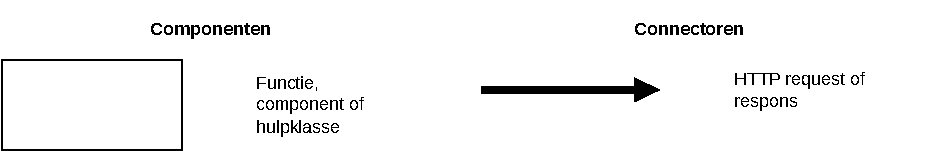
\includegraphics[width=0.8\textwidth]{../assets/images/drawio/scenario view legend.pdf}}
  \caption{Legenda voor scenario views.}
  \label{fig:scenario_view_legend}
\end{figure}

\subsection{Scenario 1: Opvragen van data}
\label{subsec:scenario_1}

Dit scenario omvat ook het opvragen van authenticatie. Dit is nodig wanneer de JWT verlopen is. Het diagram dat dit scenario beschrijft is te vinden in \autoref{fig:scenario_1}.

\begin{enumerate}
  \item De gebruiker maakt met behulp van de Authentication-hulpklasse requests naar de OIDC-provider.
  \item De OIDC-provider geeft een JWT terug.
  \item De gebruiker maak met behulp van het DeviceTable-component een request naar de API.
  \item De API stuurt een request naar de database met behulp van de gorm- en postgresbibliotheek.
  \item De database stuurt een lijst van devices terug.
  \item De API stuurt de lijst van devices terug.
  \item Het DeviceTable-component geeft de lijst met devices weer.
\end{enumerate}

\begin{figure}[ht]
  \centering
  \fbox{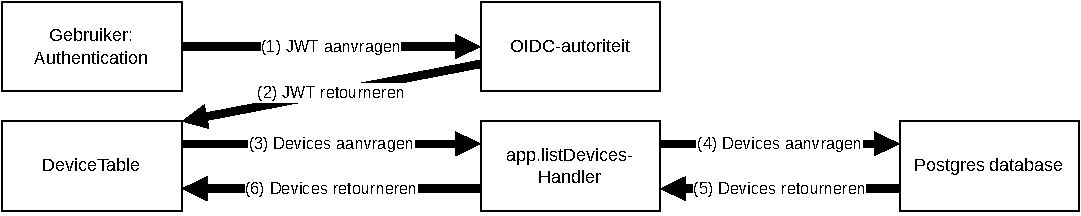
\includegraphics[width=0.8\textwidth]{../assets/images/drawio/scenario 1.pdf}}
  \caption{Scenario voor het opvragen van data.}
  \label{fig:scenario_1}
\end{figure}

\subsection{Scenario 2: Toevoegen van data}

Het diagram dat dit scenario beschrijft is te vinden in \autoref{fig:scenario_2}.

\begin{enumerate}
  \item De ondersteunende software Systemd roept het specificatieverzamelproces aan van de collector.
  \item Het specificatieverzamelproces verzamelt de specificaties.
  \item De collector stuurt met behulp van de Sender.Send-functie en de ssot-specs-api-client de specificaties van het systeem naar de API.
\end{enumerate}

\begin{figure}[ht]
  \centering
  \fbox{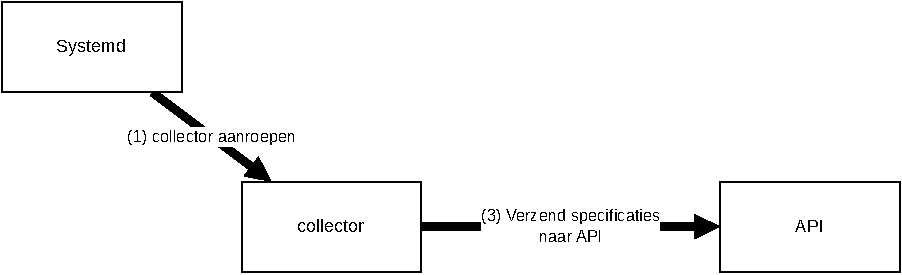
\includegraphics[width=0.8\textwidth]{../assets/images/drawio/scenario 2.pdf}}
  \caption{Scenario voor het toevoegen van data.}
  \label{fig:scenario_2}
\end{figure}

\end{document}
